\section{Cointegration}
The basic intuition of the signal is that over a given look-back window there
may exist a (temporary) \emph{cointegrating} relationship between two time
series (e.g.\ price processes, scoring rates, etc\ldots) whose expected
stability may be exploited. Formally, the cointegration property means that
there exists a linear combination (portfolio) whose implied ``spread series''
is stationary and thus has a mean and variance that do not change with time
(time-homogeneous).


\section{Strategy}
\begin{figure}
    \centering
    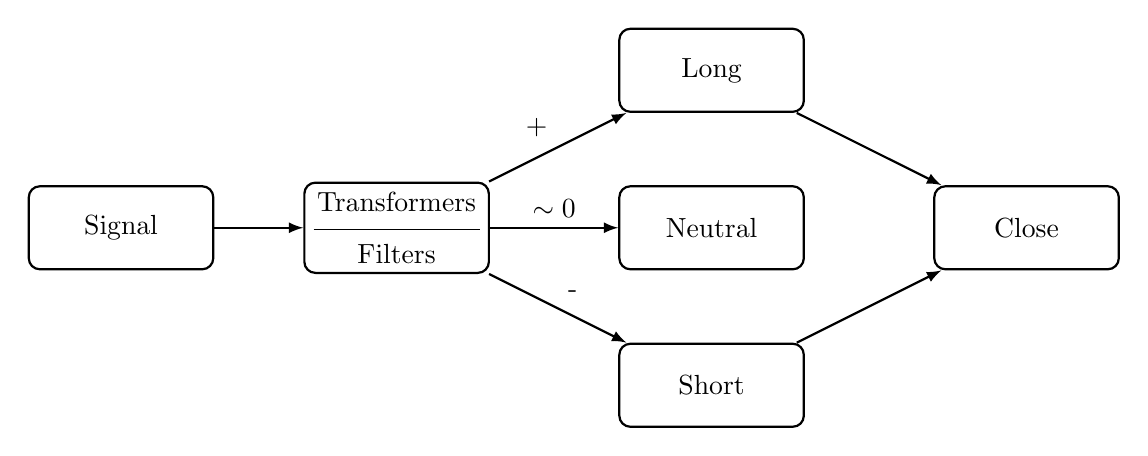
\begin{tikzpicture}[node distance=2cm, auto, thick]
        \tikzstyle{block} = [rectangle, draw, text width=6em, text centered,
        rounded corners, minimum height=3em]
        \tikzstyle{line} = [draw, -latex]

        \node [block] (node0) {Signal};
        \node [block, right of=node0, xshift=1.5cm] (node5)
            {Transformers\\[-0.5em]\noindent\rule{\linewidth}{0.6pt}\\Filters};

        \node [block, right of=node5, xshift=2cm] (node2) {Neutral};
        \node [block, above of=node2] (node1) {Long};
        \node [block, below of=node2] (node3) {Short};

        \node [block, right of=node2, xshift=2cm] (node4) {Close};

        \draw [line] (node0) -- (node5);

        \draw [line] (node5) --node {+} (node1);
        \draw [line] (node5) --node {$\sim 0$} (node2);
        \draw [line] (node5) --node {-} (node3);

        \draw [line] (node1) -- (node4);
        \draw [line] (node3) -- (node4);
    \end{tikzpicture}

    \caption{Structure of generic trading strategy which attempts to capture
    short-term trends in an asset's valuation.}\label{fig:strategy_basic}
\end{figure}

The fundamental building blocks of the strategy are very simple (see
Fig~\ref{fig:strategy_basic}):
\begin{enumerate}
    \item compute the cointegration signal;
    \item apply a sequence of filters and transformations to the signal;
    \item open a position based on the anticipated direction of the spread;
    \item close the position to lock in gains or losses.
\end{enumerate}

Each of the strategies considered herein --- for which the signals generation
processes are described in Chapter~\ref{ch:signals} --- have this structure.
The real complexity arises in the ``Signal'' and ``Transformers|Filters'' nodes
which contain our main decision making logic. For example, a typical strategy
might exploit the implied mean reversion in the spread by re-cast the spread
series into a vector of standard scores\footnote{Typically computed by
evaluating $\frac{x - \mu_x}{\sigma_x}$.} and using the current level of
deviation from the mean as an indication of the future direction; i.e.\ where a
large score would imply a negative trend due to reversion to the mean and
vice-versa.


\subsection{Interpreting signal values}
The signal, $\bm{\beta} \in \mathbb{R}$, takes the form of a real valued vector
of length $m$, where $m$ is the number of markets in the portfolio. The sign
and magnitude of each value dictates how to trade on each of the $m$ markets
(equivalently, stickers): negative values indicate short positions and, by
symmetry, positive values indicate long positions (see
Fig.~\ref{fig:signal2trade}). The absolute value is then used to assign
relative sizes to the trades in the portfolio; note that values close to zero
should likely be ignored since the resulting size is often negligible.

\begin{figure}
    \centering
    \begin{tikzpicture}[node distance=2cm]
        \node (node0) [io] {Signal $\mathbb{R}(1,)$};
        \node (node1) [decision, below of=node0, yshift=-1.5cm] {Implied bet?};

        \node (node2) [startstop, below of=node1, yshift=-1.5cm] {None};
        \node (node3) [startstop, left of=node1, xshift=-2.5cm] {Back};
        \node (node4) [startstop, right of=node1, xshift=2.5cm] {Lay};

        \draw [arrow] (node0) -- (node1);
        \draw [arrow] (node1) --node[anchor=west] {$\sim 0$} (node2);
        \draw [arrow] (node1) --node[anchor=south] {$-$} (node3);
        \draw [arrow] (node1) --node[anchor=south] {$+$} (node4);
    \end{tikzpicture}

    \caption{Illustration of generic signal to trade decision
    logic.}\label{fig:signal2trade}
\end{figure}


\subsection{Common strategy features}
\paragraph{Naming}
The cointegration strategy is written to support many underlying mechanisms for
generating a long/short signal based on an implied spread series. Further, it
arbitrarily supports any market pair for $m\geq2$. As such we need a clear
naming convention that indicates exactly \emph{what} we're trading on, and
\emph{what} method we're using to derive the signal. The following conventions
are imposed:
\begin{description}[leftmargin=!, labelwidth=8em]
    \item[\mintinline{python}{strategy_name}] For readability, it is suggested
        that the strategy name include ``coint''. For now the only concrete
        implementation of the strategy, based on market price processes, has
        the name: \textbf{coint\_mpc}.
    \item[\mintinline{python}{strategy_desc}] The strategy descriptor defines
        the method used inside the signal generator to extract a direction
        (prediction) from the spread series.
    \item[\mintinline{python}{strategy_code}] The strategy code should be used to add final details to the cointegration strategy such as which market to trade on.
    \item[\mintinline{python}{mnemonic}] This can be used to distinguish even
        further in case you wanted to do some specific tests, say with
        \mintinline{python}{MatchingMode.ALWAYS_MATCH}. Though the value of
        \mintinline{python}{mnemonic} does not affect anything in the code, it
        does allow for manual debugging and filtering in the database.
\end{description}


\paragraph{Parameters}
Though each iteration of the cointegration strategy may have it's own set of
parameters, some are common throughout:
\begin{description}[leftmargin=!, labelwidth=2em]
    \item[\mintinline{python}{LB}] the number of periods to include in the
        look-back window.
    \item[\mintinline{python}{SS}] the sub-sampling rate for the look-back
        window; i.e.\ for a value 2, we sample every other value\footnote{The
            sub-sampling rate is especially important when using
            computationally intensive methods for predicting changes in the
            spread series. For our purposes this will not be the case, though
        it is still informative to investigate it's impact on returns.}.
    \item[$\underbar{$t$}$] the minimum holding time for a given portfolio;
        for practical reasons this is lower bounded by the in-play delay.
    \item[$T$] the maximum holding time for a given portfolio; this is only
        comes into effect when no non-zero signal is observed.
    \item[$r_\text{TP}$] The take-profit threshold on expected portfolio
        returns.
    \item[$r_\text{SL}$] The stop-loss threshold on expected portfolio
        returns.
\end{description}


\begin{figure}
    \centering
    \begin{tikzpicture}[node distance=2cm]
        \node (node2) [io] {Signal $\mathbb{R}(1, m)$};
        \node (node3) [decision, below of=node2, yshift=-1.5cm] {Active portfolio exists?};

        \node (node11) [decision, below of=node3, yshift=-3cm] {Within odds bounds?};
        \node (node12) [startstop, left of=node11, xshift=-3cm] {Ignore};

        \node (node4) [decision, right of=node3, xshift=3cm] {Signals conflict?};
        \node (node8) [process, right of=node11, xshift=3cm] {Close portfolio};
        \node (node7) [startstop, above of=node4, yshift=1.5cm] {Ignore};

        \node (node9) [process, below of=node11, yshift=-1.5cm] {Open portfolio};
        \node (node10) [startstop, below of=node9] {Done};

        \draw [arrow] (node3) --node[anchor=south] {Y} (node4);
        \draw [arrow] (node4) --node[anchor=east] {N} (node7);

        \draw [arrow] (node3) --node[anchor=east] {N} (node11);
        \draw [arrow] (node2) -- (node3);
        \draw [arrow] (node8) -- (node11);
        \draw [arrow] (node4) --node[anchor=east] {Y} (node8);

        \draw [arrow] (node9) -- (node10);
        \draw [arrow] (node11) --node[anchor=south] {N} (node12);
        \draw [arrow] (node11) --node[anchor=east] {Y} (node9);
    \end{tikzpicture}

    \caption{\todo[inline]{Add description of this diagram and why it's common
    to all strategies.}}
\end{figure}

\begin{figure}
    \centering
    \begin{tikzpicture}[node distance=2cm]
        \node (node0) [io] {Tick};
        \node (node1) [process, below of=node0] {Update portfolios};

        \node (node2) [decision, right of=node1, xshift=3cm] {$t < \underbar{$t$}$};
        \node (node3) [decision, below of=node2, yshift=-2cm] {$r_t > r_\text{TP}$};
        \node (node4) [decision, below of=node3, yshift=-2cm] {$r_t < r_\text{SL}$};
        \node (node5) [decision, below of=node4, yshift=-2cm] {$t > T$};

        \node (node6) [startstop, right of=node2, xshift=3cm] {Done};
        \node (node7) [startstop, right of=node4, xshift=3cm] {Close portfolio};
        \node (node8) [startstop, left of=node5, xshift=-3cm] {Done};

        \draw [arrow] (node0) -- (node1);
        \draw [arrow] (node1) -- (node2);

        \draw [arrow] (node2) --node[anchor=south] {Y} (node6);
        \draw [arrow] (node3) --node[anchor=south] {Y} (node7);
        \draw [arrow] (node4) --node[anchor=south] {Y} (node7);
        \draw [arrow] (node5) --node[anchor=south] {Y} (node7);

        \draw [arrow] (node2) --node[anchor=west] {N} (node3);
        \draw [arrow] (node3) --node[anchor=west] {N} (node4);
        \draw [arrow] (node4) --node[anchor=west] {N} (node5);
        \draw [arrow] (node5) --node[anchor=south] {N} (node8);
    \end{tikzpicture}

    \caption{\todo[inline]{Add description of this diagram and why it's common
    to all strategies.}}
\end{figure}
